% https://www.overleaf.com/
\documentclass[tikz,border=20pt]{standalone}
\usepackage{tikz}
\usetikzlibrary{trees, positioning, arrows.meta, decorations.pathmorphing, matrix}

\begin{document}

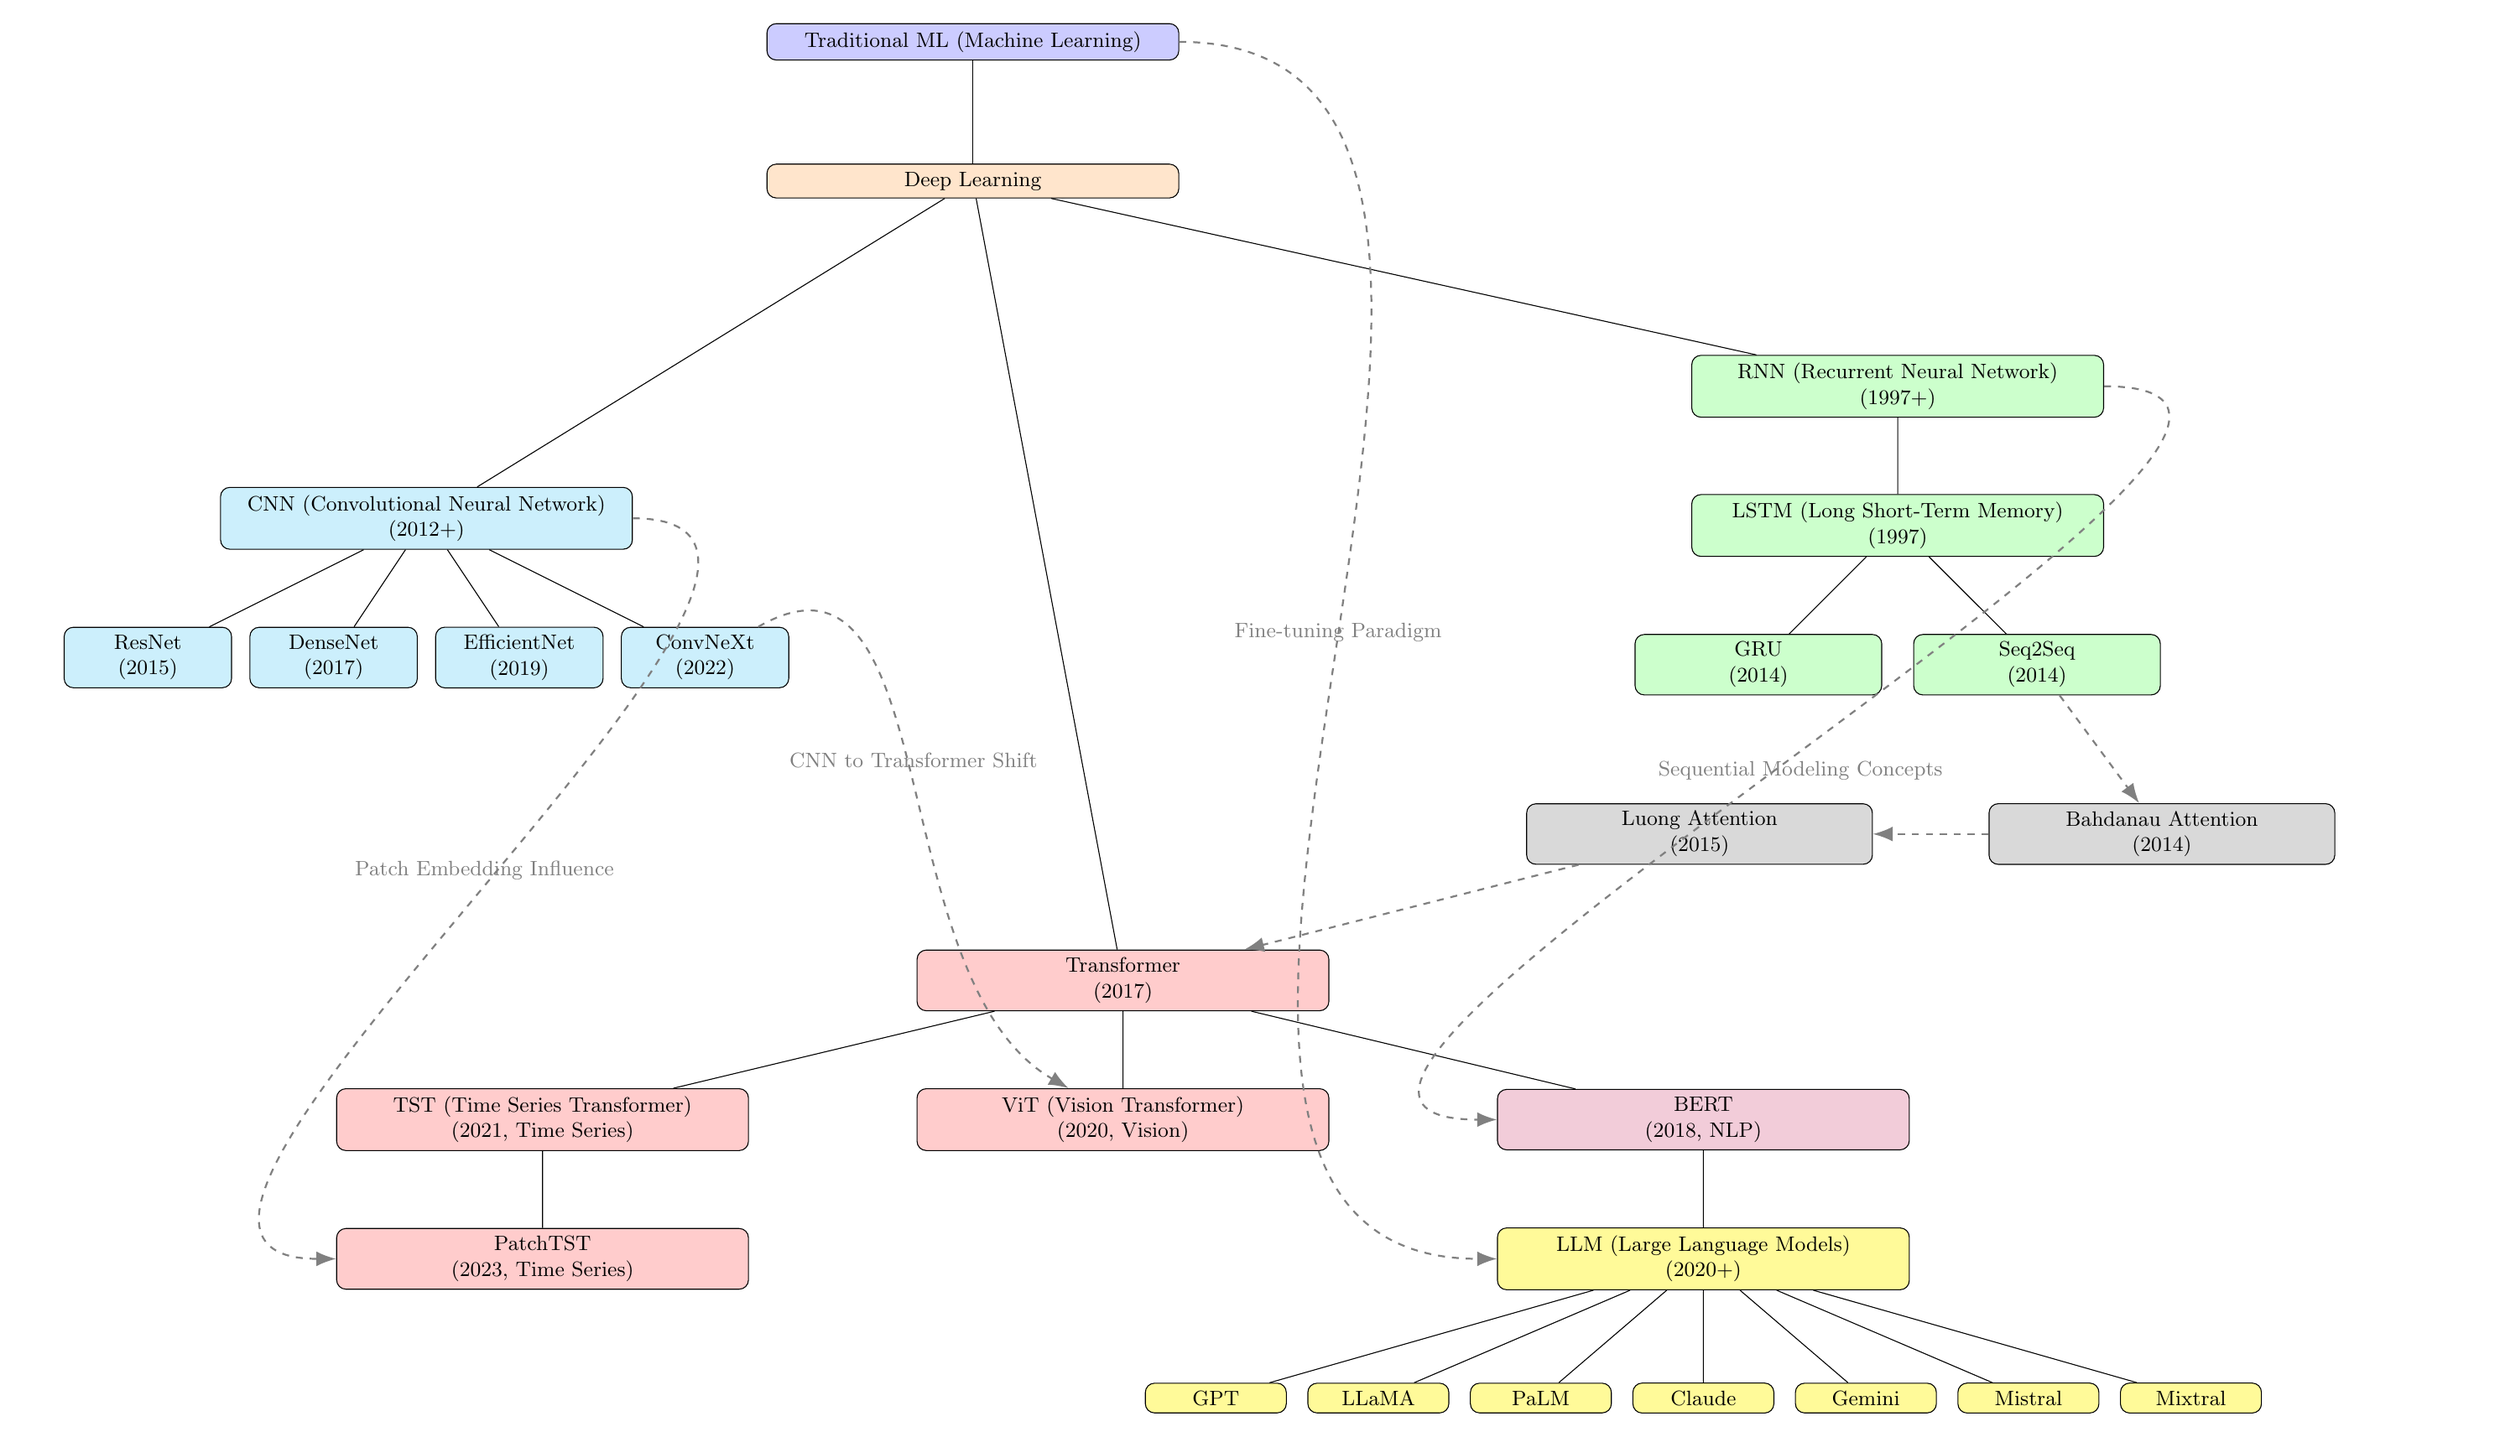
\begin{tikzpicture}[
  sibling distance=15em,
  level distance=6em,
  every node/.style={font=\small, align=center},
  ml/.style={rectangle, draw=black, fill=blue!20, rounded corners, text width=6cm},
  dl/.style={rectangle, draw=black, fill=orange!20, rounded corners, text width=6cm},
  rnn/.style={rectangle, draw=black, fill=green!20, rounded corners, text width=6cm},
  rnnchild/.style={rnn, text width=3.5cm},
  cnn/.style={rectangle, draw=black, fill=cyan!20, rounded corners, text width=6cm},
  cnnchild/.style={cnn, text width=2.3cm},
  nlp/.style={rectangle, draw=black, fill=purple!20, rounded corners, text width=6cm},
  tst/.style={rectangle, draw=black, fill=red!20, rounded corners, text width=6cm},
  llm/.style={rectangle, draw=black, fill=yellow!40, rounded corners, text width=6cm},
  llmchild/.style={llm, text width=1.9cm},
  att/.style={rectangle, draw=black, fill=gray!30, rounded corners, text width=5cm},
  >={Latex[length=3mm]}
]

% 트리 구조 시작
\node[ml] (ml) {Traditional ML (Machine Learning)}
  child {node[dl] (dl) {Deep Learning}
    child[shift={(-3,-3)}] {node[cnn] (cnn) {CNN (Convolutional Neural Network)\\(2012+)}
      [sibling distance=8em]
      child {node[cnnchild] {ResNet\\(2015)}}
      child {node[cnnchild] {DenseNet\\(2017)}}
      child {node[cnnchild] {EfficientNet\\(2019)}}
      child {node[cnnchild] (convnext) {ConvNeXt\\(2022)}}
    }
    child[shift={(14,-1)}] {node[rnn] (rnn) {RNN (Recurrent Neural Network)\\(1997+)}
      child {node[rnn] (lstm) {LSTM (Long Short-Term Memory)\\(1997)}
        [sibling distance=12em]
        child {node[rnnchild] {GRU\\(2014)}}
        child {node[rnnchild] (seq2seq) {Seq2Seq\\(2014)}}
      }
    }
    child[shift={(-3,-10)}] {node[tst] (transformer) {Transformer\\(2017)}
      [sibling distance=25em]
      child {node[tst] (tst) {TST (Time Series Transformer)\\(2021, Time Series)}
        child {node[tst] (patch) {PatchTST\\(2023, Time Series)}}
      }
      child {node[tst] (vit) {ViT (Vision Transformer)\\(2020, Vision)}}
      child {node[nlp] (bert) {BERT\\(2018, NLP)}
        child {node[llm] (llm) {LLM (Large Language Models)\\(2020+)}
          [sibling distance=7em]
          child {node[llmchild] {GPT}}
          child {node[llmchild] {LLaMA}}
          child {node[llmchild] {PaLM}}
          child {node[llmchild] {Claude}}
          child {node[llmchild] {Gemini}}
          child {node[llmchild] {Mistral}}
          child {node[llmchild] {Mixtral}}
        }}
    }
  };

% Attention 계열 모델 분기
\node[att] (bahdanau) at (18,-12) {Bahdanau Attention\\(2014)};
\node[att] (luong) at (11,-12) {Luong Attention\\(2015)};
\draw[dashed,->,thick,gray] (seq2seq) -- (bahdanau);
\draw[dashed,->,thick,gray] (bahdanau) -- (luong);
\draw[dashed,->,thick,gray] (luong) -- (transformer);

% 영향선 (dashed arrows)
\draw[dashed,->,thick,gray] (cnn) to[out=0,in=180] node[midway, above, font=\small]{Patch Embedding Influence} (patch);
\draw[dashed,->,thick,gray] (rnn) to[out=0,in=180] node[midway, below, font=\small]{Sequential Modeling Concepts} (bert);
\draw[dashed,->,thick,gray] (ml) to[out=0,in=180] node[midway, above, font=\small]{Fine-tuning Paradigm} (llm);
\draw[dashed,->,thick,gray] (convnext) to[out=30,in=150] node[midway, above, font=\small]{CNN to Transformer Shift} (vit);

% (선택) 전설 추가 가능

\end{tikzpicture}

\end{document}
